% LaTeX source for ``Python for Informatics: Exploring Information''
% Copyright (c)  2010  Charles R. Severance

% Permission is granted to copy, distribute and/or modify this
% document under the terms of the 
% 
% Creative Commons Attribution 3.0 - Share Alike Unported
% (or a later CC-SA) license

% http://creativecommons.org/licenses/by-sa/3.0/

\chapter{Advanced functions}
\label{fruitchap}

\section{Return values}
\index{return value}

Some of the built-in functions we have used, such as the math
functions, produce results.  Calling the function generates a
value, which we usually assign to a variable or use as part of an
expression.

\beforeverb
\begin{verbatim}
e = math.exp(1.0)
height = radius * math.sin(radians)
\end{verbatim}
\afterverb
%
All of the functions we have written so far are void; they print
something or move turtles around, but their return value is {\tt
None}.

In this chapter, we are (finally) going to write fruitful functions.
The first example is {\tt area}, which returns the area of a circle
with the given radius:

\beforeverb
\begin{verbatim}
def area(radius):
    temp = math.pi * radius**2
    return temp
\end{verbatim}
\afterverb
%
We have seen the {\tt return} statement before, but in a fruitful
function the {\tt return} statement includes
an expression.  This statement means: ``Return immediately from
this function and use the following expression as a return value.''
The expression can be arbitrarily complicated, so we could
have written this function more concisely:

\index{return statement}
\index{statement!return}

\beforeverb
\begin{verbatim}
def area(radius):
    return math.pi * radius**2
\end{verbatim}
\afterverb
%
On the other hand, {\bf temporary variables} like {\tt temp} often make
debugging easier.

\index{temporary variable}
\index{variable!temporary}

Sometimes it is useful to have multiple return statements, one in each
branch of a conditional:

\beforeverb
\begin{verbatim}
def absolute_value(x):
    if x < 0:
        return -x
    else:
        return x
\end{verbatim}
\afterverb
%
Since these {\tt return} statements are in an alternative conditional,
only one will be executed.

As soon as a return statement executes, the function
terminates without executing any subsequent statements.
Code that appears after a {\tt return} statement, or any other place
the flow of execution can never reach, is called {\bf dead code}.

\index{dead code}

In a fruitful function, it is a good idea to ensure
that every possible path through the program hits a
{\tt return} statement.  For example:

\beforeverb
\begin{verbatim}
def absolute_value(x):
    if x < 0:
        return -x
    if x > 0:
        return x
\end{verbatim}
\afterverb
%
This function is incorrect because if {\tt x} happens to be 0,
neither condition is true, and the function ends without hitting a
{\tt return} statement.  If the flow of execution gets to the end
of a function, the return value is {\tt None}, which is not
the absolute value of 0.

\index{None special value}
\index{special value!None}

\beforeverb
\begin{verbatim}
>>> print absolute_value(0)
None
\end{verbatim}
\afterverb
%
By the way, Python provides a built-in function called 
{\tt abs} that computes absolute values.

\index{abs function}
\index{function!abs}

\begin{ex}

\index{compare function}
\index{function!compare}

Write a {\tt compare} function
that returns {\tt 1} if {\tt x > y},
{\tt 0} if {\tt x == y}, and {\tt -1} if {\tt x < y}.
\end{ex}

\section{Tuples as return values}

\index{tuple}
\index{value!tuple}
\index{return value!tuple}
\index{function, tuple as return value}

Strictly speaking, a function can only return one value, but
if the value is a tuple, the effect is the same as returning
multiple values.  For example, if you want to divide two integers
and compute the quotient and remainder, it is inefficient to
compute {\tt x/y} and then {\tt x\%y}.  It is better to compute
them both at the same time.

\index{divmod}

The built-in function {\tt divmod} takes two arguments and
returns a tuple of two values, the quotient and remainder.
You can store the result as a tuple:

\beforeverb
\begin{verbatim}
>>> t = divmod(7, 3)
>>> print t
(2, 1)
\end{verbatim}
\afterverb
%
Or use tuple assignment to store the elements separately:

\index{tuple assignment}
\index{assignment!tuple}

\beforeverb
\begin{verbatim}
>>> quot, rem = divmod(7, 3)
>>> print quot
2
>>> print rem
1
\end{verbatim}
\afterverb
%
Here is an example of a function that returns a tuple:

\beforeverb
\begin{verbatim}
def min_max(t):
    return min(t), max(t)
\end{verbatim}
\afterverb
%
{\tt max} and {\tt min} are built-in functions that find
the largest and smallest elements of a sequence.  \verb"min_max"
computes both and returns a tuple of two values.

\index{max function}
\index{function!max}
\index{min function}
\index{function!min}


\section{Variable-length argument tuples}

\index{variable-length argument tuple}
\index{argument!variable-length tuple}
\index{gather}
\index{parameter!gather}
\index{argument!gather}

Functions can take a variable number of arguments.  A parameter
name that begins with {\tt *} {\bf gathers} arguments into
a tuple.  For example, {\tt printall}
takes any number of arguments and prints them:

\beforeverb
\begin{verbatim}
def printall(*args):
    print args
\end{verbatim}
\afterverb
%
The gather parameter can have any name you like, but {\tt args} is
conventional.  Here's how the function works:

\beforeverb
\begin{verbatim}
>>> printall(1, 2.0, '3')
(1, 2.0, '3')
\end{verbatim}
\afterverb
%
You can combine the gather operator with required and positional
arguments:

\beforeverb
\begin{verbatim}
def pointless(required, optional=0, *args):
    print required, optional, args
\end{verbatim}
\afterverb
%
Run this function with 1, 2, 3 and 4 or more arguments and
make sure you understand what it does.

\index{scatter}
\index{argument scatter}

The complement of gather is {\bf scatter}.  If you have a
sequence of values and you want to pass it to a function
as multiple arguments, you can use the {\tt *} operator.
For example, {\tt divmod} takes exactly two arguments; it
doesn't work with a tuple:

\index{TypeError}
\index{exception!TypeError}

\beforeverb
\begin{verbatim}
>>> t = (7, 3)
>>> divmod(t)
TypeError: divmod expected 2 arguments, got 1
\end{verbatim}
\afterverb
%
But if you scatter the tuple, it works:

\beforeverb
\begin{verbatim}
>>> divmod(*t)
(2, 1)
\end{verbatim}
\afterverb
%

\begin{ex}
Many of the built-in functions use
variable-length argument tuples.  For example, {\tt max}
and {\tt min} can take any number of arguments:

\index{max function}
\index{function!max}
\index{min function}
\index{function!min}

\beforeverb
\begin{verbatim}
>>> max(1,2,3)
3
\end{verbatim}
\afterverb
%
But {\tt sum} does not.

\index{sum function}
\index{function!sum}

\beforeverb
\begin{verbatim}
>>> sum(1,2,3)
TypeError: sum expected at most 2 arguments, got 3
\end{verbatim}
\afterverb
%
Write a function called {\tt sumall} that takes any number
of arguments and returns their sum.

\end{ex}



\section{Variables and parameters are local}
\index{local variable}
\index{variable!local}

When you create a variable inside a function, it is {\bf local},
which means that it only
exists inside the function.  For example:

\index{parentheses!parameters in}

\beforeverb
\begin{verbatim}
def cat_twice(part1, part2):
    cat = part1 + part2
    print_twice(cat)
\end{verbatim}
\afterverb
%
This function takes two arguments, concatenates them, and prints
the result twice.  Here is an example that uses it:

\index{concatenation}

\beforeverb
\begin{verbatim}
>>> line1 = 'Bing tiddle '
>>> line2 = 'tiddle bang.'
>>> cat_twice(line1, line2)
Bing tiddle tiddle bang.
Bing tiddle tiddle bang.
\end{verbatim}
\afterverb
%
When \verb"cat_twice" terminates, the variable {\tt cat}
is destroyed.  If we try to print it, we get an exception:

\index{NameError}
\index{exception!NameError}

\beforeverb
\begin{verbatim}
>>> print cat
NameError: name 'cat' is not defined
\end{verbatim}
\afterverb
%
Parameters are also local.
For example, outside \verb"print_twice", there is no
such thing as {\tt bruce}.

\index{parameter}

\section{Global variables}

\index{global variable}
\index{variable!global}

In the previous example, {\tt known} is created outside the function,
so it belongs to the special frame called \verb"__main__".
Variables in \verb"__main__" are sometimes called {\bf global}
because they can be accessed from any function.  Unlike local
variables, which disappear when their function ends, global variables
persist from one function call to the next.

\index{flag}

It is common to use global variables for {\bf flags}; that is, 
boolean variables that indicate (``flag'') whether a condition
is true.  For example, some programs use
a flag named {\tt verbose} to control the level of detail in the
output:

\beforeverb
\begin{verbatim}
verbose = True

def example1():
    if verbose:
        print 'Running example1'
\end{verbatim}
\afterverb
%
If you try to reassign a global variable, you might be surprised.
The following example is supposed to keep track of whether the
function has been called:

\index{multiple assignment}
\index{assignment!multiple}

\beforeverb
\begin{verbatim}
been_called = False

def example2():
    been_called = True         # WRONG
\end{verbatim}
\afterverb
%
But if you run it you will see that the value of \verb"been_called"
doesn't change.  The problem is that {\tt example2} creates a new local
variable named \verb"been_called".  The local variable goes away when
the function ends, and has no effect on the global variable.

\index{global statement}
\index{statement!global}
\index{declaration}

To reassign a global variable inside a function you have to
{\bf declare} the global variable before you use it:

\beforeverb
\begin{verbatim}
been_called = False

def example2():
    global been_called 
    been_called = True
\end{verbatim}
\afterverb
%
The {\tt global} statement tells the interpreter
something like, ``In this function, when I say \verb"been_called", I
mean the global variable; don't create a local one.''

\index{update!global variable}
\index{global variable!update}

Here's an example that tries to update a global variable:

\beforeverb
\begin{verbatim}
count = 0

def example3():
    count = count + 1          # WRONG
\end{verbatim}
\afterverb
%
If you run it you get:

\index{UnboundLocalError}
\index{exception!UnboundLocalError}

\beforeverb
\begin{verbatim}
UnboundLocalError: local variable 'count' referenced before assignment
\end{verbatim}
\afterverb
%
Python assumes that {\tt count} is local, which means
that you are reading it before writing it.  The solution, again,
is to declare {\tt count} global.

\index{counter}

\beforeverb
\begin{verbatim}
def example3():
    global count
    count += 1
\end{verbatim}
\afterverb
%
If the global value is mutable, you can modify it without
declaring it:

\index{mutability}

\beforeverb
\begin{verbatim}
known = {0:0, 1:1}

def example4():
    known[2] = 1
\end{verbatim}
\afterverb
%
So you can add, remove and replace elements of a global list or
dictionary, but if you want to reassign the variable, you
have to declare it:

\beforeverb
\begin{verbatim}
def example5():
    global known
    known = dict()
\end{verbatim}
\afterverb
%

\section{Incremental development}
\label{incremental development}
\index{development plan!incremental}

As you write larger functions, you might find yourself
spending more time debugging.

To deal with increasingly complex programs,
you might want to try a process called
{\bf incremental development}.  The goal of incremental development
is to avoid long debugging sessions by adding and testing only
a small amount of code at a time.

\index{testing!incremental development}
\index{Pythagorean theorem}

As an example, suppose you want to find the distance between two
points, given by the coordinates $(x_1, y_1)$ and $(x_2, y_2)$.
By the Pythagorean theorem, the distance is:

\begin{displaymath}
\mathrm{distance} = \sqrt{(x_2 - x_1)^2 + (y_2 - y_1)^2}
\end{displaymath}
%
The first step is to consider what a {\tt distance} function should
look like in Python.  In other words, what are the inputs (parameters)
and what is the output (return value)?

In this case, the inputs are two points, which you can represent
using four numbers.  The return value is the distance, which is
a floating-point value.

Already you can write an outline of the function:

\beforeverb
\begin{verbatim}
def distance(x1, y1, x2, y2):
    return 0.0
\end{verbatim}
\afterverb
%
Obviously, this version doesn't compute distances; it always returns
zero.  But it is syntactically correct, and it runs, which means that
you can test it before you make it more complicated.

To test the new function, call it with sample arguments:

\beforeverb
\begin{verbatim}
>>> distance(1, 2, 4, 6)
0.0
\end{verbatim}
\afterverb
%
I chose these values so that the horizontal distance is 3 and the
vertical distance is 4; that way, the result is 5
(the hypotenuse of a 3-4-5 triangle). When testing a function, it is
useful to know the right answer.

\index{testing!knowing the answer}

At this point we have confirmed that the function is syntactically
correct, and we can start adding code to the body.
A reasonable next step is to find the differences
$x_2 - x_1$ and $y_2 - y_1$.  The next version stores those values in
temporary variables and prints them.

\beforeverb
\begin{verbatim}
def distance(x1, y1, x2, y2):
    dx = x2 - x1
    dy = y2 - y1
    print 'dx is', dx
    print 'dy is', dy
    return 0.0
\end{verbatim}
\afterverb
%
If the function is working, it should display \verb"'dx is 3'" and {\tt
'dy is 4'}.  If so, we know that the function is getting the right
arguments and performing the first computation correctly.  If not,
there are only a few lines to check.

Next we compute the sum of squares of {\tt dx} and {\tt dy}:

\beforeverb
\begin{verbatim}
def distance(x1, y1, x2, y2):
    dx = x2 - x1
    dy = y2 - y1
    dsquared = dx**2 + dy**2
    print 'dsquared is: ', dsquared
    return 0.0
\end{verbatim}
\afterverb
%
Again, you would run the program at this stage and check the output
(which should be 25).
Finally, you can use {\tt math.sqrt} to compute and return the result:

\index{sqrt}
\index{function!sqrt}

\beforeverb
\begin{verbatim}
def distance(x1, y1, x2, y2):
    dx = x2 - x1
    dy = y2 - y1
    dsquared = dx**2 + dy**2
    result = math.sqrt(dsquared)
    return result
\end{verbatim}
\afterverb
%
If that works correctly, you are done.  Otherwise, you might
want to print the value of {\tt result} before the return
statement.

The final version of the function doesn't display anything when it
runs; it only returns a value.  The {\tt print} statements we wrote
are useful for debugging, but once you get the function working, you
should remove them.  Code like that is called {\bf scaffolding}
because it is helpful for building the program but is not part of the
final product.

\index{scaffolding}

When you start out, you should add only a line or two of code at a
time.  As you gain more experience, you might find yourself writing
and debugging bigger chunks.  Either way, incremental development
can save you a lot of debugging time.

The key aspects of the process are:

\begin{enumerate}

\item Start with a working program and make small incremental changes. 
At any point, if there is an error, you should have a good idea
where it is.

\item Use temporary variables to hold intermediate values so you can
display and check them.

\item Once the program is working, you might want to remove some of
the scaffolding or consolidate multiple statements into compound
expressions, but only if it does not make the program difficult to
read.

\end{enumerate}

\begin{ex}

\index{hypotenuse}

Use incremental development to write a function
called {\tt hypotenuse} that returns the length of the hypotenuse of a
right triangle given the lengths of the two legs as arguments.
Record each stage of the development process as you go.
\end{ex}


\section{Composition}

\index{composition}
\index{function composition}

As you should expect by now, you can call one function from
within another.  This ability is called {\bf composition}.

As an example, we'll write a function that takes two points,
the center of the circle and a point on the perimeter, and computes
the area of the circle.

Assume that the center point is stored in the variables {\tt xc} and
{\tt yc}, and the perimeter point is in {\tt xp} and {\tt yp}. The
first step is to find the radius of the circle, which is the distance
between the two points.  We just wrote a function, {\tt
distance}, that does that:

\beforeverb
\begin{verbatim}
radius = distance(xc, yc, xp, yp)
\end{verbatim}
\afterverb
%
The next step is to find the area of a circle with that radius;
we just wrote that, too:

\beforeverb
\begin{verbatim}
result = area(radius)
\end{verbatim}
\afterverb
%
Encapsulating these steps in a function, we get:

\index{encapsulation}

\beforeverb
\begin{verbatim}
def circle_area(xc, yc, xp, yp):
    radius = distance(xc, yc, xp, yp)
    result = area(radius)
    return result
\end{verbatim}
\afterverb
%
The temporary variables {\tt radius} and {\tt result} are useful for
development and debugging, but once the program is working, we can
make it more concise by composing the function calls:

\beforeverb
\begin{verbatim}
def circle_area(xc, yc, xp, yp):
    return area(distance(xc, yc, xp, yp))
\end{verbatim}
\afterverb
%

\section{Stack diagrams}
\label{stackdiagram}
\index{stack diagram}
\index{function frame}
\index{frame}

To keep track of which variables can be used where, it is sometimes
useful to draw a {\bf stack diagram}.  Like state diagrams, stack
diagrams show the value of each variable, but they also show the
function each variable belongs to.

\index{stack diagram}
\index{diagram!stack}

Each function is represented by a {\bf frame}.  A frame is a box
with the name of a function
beside it and the parameters and variables of the function inside it.
The stack diagram for the
previous example looks like this:

\beforefig
\centerline{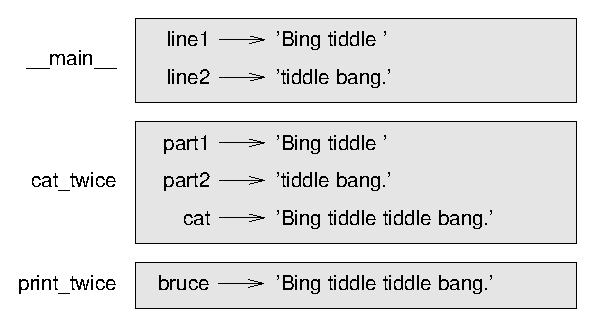
\includegraphics{figs/stack.eps}}
\afterfig

The frames are arranged in a stack that indicates which function
called which, and so on.  In this example, \verb"print_twice"
was called by \verb"cat_twice", and \verb"cat_twice" was called by 
\verb"__main__", which is a special name for the topmost frame.  When
you create a variable outside of any function, it belongs to 
\verb"__main__".

Each parameter refers to the same value as its corresponding
argument.  So, {\tt part1} has the same value as
{\tt line1}, {\tt part2} has the same value as {\tt line2},
and {\tt bruce} has the same value as {\tt cat}.

If an error occurs during a function call, Python prints the
name of the function, and the name of the function that called
it, and the name of the function that called {\em that}, all the
way back to \verb"__main__".

For example, if you try to access {\tt cat} from within 
\verb"print_twice", you get a {\tt NameError}:

\beforeverb
\begin{verbatim}
Traceback (innermost last):
  File "test.py", line 13, in __main__
    cat_twice(line1, line2)
  File "test.py", line 5, in cat_twice
    print_twice(cat)
  File "test.py", line 9, in print_twice
    print cat
NameError: name 'cat' is not defined
\end{verbatim}
\afterverb
%
This list of functions is called a {\bf traceback}.  It tells you what
program file the error occurred in, and what line, and what functions
were executing at the time.  It also shows the line of code that
caused the error.

\index{traceback}

The order of the functions in the traceback is the same as the
order of the frames in the stack diagram.  The function that is
currently running is at the bottom.


\section{Boolean functions}
\label{boolean}

\index{boolean function}

Functions can return booleans, which is often convenient for hiding
complicated tests inside functions.  For example:

\beforeverb
\begin{verbatim}
def is_divisible(x, y):
    if x % y == 0:
        return True
    else:
        return False
\end{verbatim}
\afterverb
%
It is common to give boolean functions names that sound like yes/no
questions; \verb"is_divisible" returns either {\tt True} or {\tt False}
to indicate whether {\tt x} is divisible by {\tt y}.

Here is an example:

\beforeverb
\begin{verbatim}
>>>   is_divisible(6, 4)
False
>>>   is_divisible(6, 3)
True
\end{verbatim}
\afterverb
%
The result of the {\tt ==} operator is a boolean, so we can write the
function more concisely by returning it directly:

\beforeverb
\begin{verbatim}
def is_divisible(x, y):
    return x % y == 0
\end{verbatim}
\afterverb
%
Boolean functions are often used in conditional statements:

\index{conditional statement}
\index{statement!conditional}

\beforeverb
\begin{verbatim}
if is_divisible(x, y):
    print 'x is divisible by y'
\end{verbatim}
\afterverb
%
It might be tempting to write something like:

\beforeverb
\begin{verbatim}
if is_divisible(x, y) == True:
    print 'x is divisible by y'
\end{verbatim}
\afterverb
%
But the extra comparison is unnecessary.

\begin{ex}
Write a function \verb"is_between(x, y, z)" that
returns {\tt True} if $x \le y \le z$ or {\tt False} otherwise.
\end{ex}

\section{Optional parameters}

\index{optional parameter}
\index{parameter!optional}

We have seen built-in functions and methods that take a variable
number of arguments.  It is possible to write user-defined functions
with optional arguments, too.  For example, here is a function that
prints the most common words in a histogram

\beforeverb
\begin{verbatim}
def print_most_common(hist, num=10)
    t = most_common(hist)
    print 'The most common words are:'
    for freq, word in t[0:num]:
        print word, '\t', freq
\end{verbatim}
\afterverb

The first parameter is required; the second is optional.
The {\bf default value} of {\tt num} is 10.

\index{default value}
\index{value!default}

If you only provide one argument:

\beforeverb
\begin{verbatim}
print_most_common(hist)
\end{verbatim}
\afterverb

{\tt num} gets the default value.  If you provide two arguments:

\beforeverb
\begin{verbatim}
print_most_common(hist, 20)
\end{verbatim}
\afterverb

{\tt num} gets the value of the argument instead.  In other
words, the optional argument {\bf overrides} the default value.

\index{override}

If a function has both required and optional parameters, all
the required parameters have to come first, followed by the
optional ones.

% TBD - May want to talk about "guarding" code here - lots removed

\section{Debugging}
\label{factdebug}

\index{debugging}

Breaking a large program into smaller functions creates natural
checkpoints for debugging.  If a function is not working, there are
three possibilities to consider:

\begin{itemize}

\item There is something wrong with the arguments the function
is getting; a precondition is violated.

\item There is something wrong with the function; a postcondition
is violated.

\item There is something wrong with the return value or the
way it is being used.

\end{itemize}

To rule out the first possibility, you can add a {\tt print} statement
at the beginning of the function and display the values of the
parameters (and maybe their types).  Or you can write code
that checks the preconditions explicitly.

\index{precondition}
\index{postcondition}

If the parameters look good, add a {\tt print} statement before each
{\tt return} statement that displays the return value.  If
possible, check the result by hand.  Consider calling the
function with values that make it easy to check the result
(as in Section~\ref{incremental development}).

If the function seems to be working, look at the function call
to make sure the return value is being used correctly (or used
at all!).

\index{flow of execution}

Adding print statements at the beginning and end of a function
can help make the flow of execution more visible.

If you are confused about the flow of execution, this kind of
output can be helpful.  It takes some time to develop effective
scaffolding, but a little bit of scaffolding can save a lot of debugging.


\section{Glossary}

\begin{description}

\item[call graph:] A diagram that shows every frame created during
the execution of a program, with an arrow from each caller to
each callee. 

\index{call graph}
\index{diagram!call graph}

\item[dead code:]  Part of a program that can never be executed, often because
it appears after a {\tt return} statement.
\index{dead code}

\item[declaration:] A statement like {\tt global} that tells the
interpreter something about a variable.
\index{declaration}

\item[default value:] The value given to an optional parameter if no
argument is provided.
\index{default value}

\item[flag:] A boolean variable used to indicate whether a condition
is true.
\index{flag}

\item[frame:]  A box in a stack diagram that represents a function call.
It contains the local variables and parameters of the function.
\index{function frame}
\index{frame}

\item[global variable:]  A variable defined outside a function.  Global
variables can be accessed from any function.
\index{global variable}

\item[guardian:]  A programming pattern that uses a conditional
statement to check for and handle circumstances that
might cause an error.
\index{guardian pattern}
\index{pattern!guardian}

\item[incremental development:]  A program development plan intended to
avoid debugging by adding and testing only
a small amount of code at a time.
\index{incremental development}

\item[local variable:]  A variable defined inside a function.  A local
variable can only be used inside its function.
\index{local variable}

\item[{\tt None}:]  A special value returned by functions that
have no return statement or a return statement without an argument.
\index{None special value}
\index{special value!None}

\item[override:] To replace a default value with an argument.
\index{override}

\item[scaffolding:]  Code that is used during program development but is
not part of the final version.
\index{scaffolding}

\item[stack diagram:]  A graphical representation of a stack of functions,
their variables, and the values they refer to.
\index{stack diagram}

\item[temporary variable:]  A variable used to store an intermediate value in
a complex calculation.
\index{temporary variable}
\index{variable!temporary}

\item[traceback:]  A list of the functions that are executing,
printed when an exception occurs.
\index{traceback}


\end{description}


\section{Exercises}

\begin{ex}
\index{stack diagram}

Draw a stack diagram for the following
program.  What does the program print?

\beforeverb
\begin{verbatim}
def b(z):
    prod = a(z, z)
    print z, prod
    return prod

def a(x, y):
    x = x + 1
    return x * y

def c(x, y, z):
    sum = x + y + z
    pow = b(sum)**2
    return pow

x = 1
y = x + 1
print c(x, y+3, x+y)
\end{verbatim}
\afterverb

\end{ex}



\begin{ex}
\label{palindrome}

\index{palindrome}

A palindrome is a word that is spelled the same backward and
forward, like ``noon'' and ``redivider''.  Recursively, a word
is a palindrome if the first and last letters are the same
and the middle is a palindrome.

The following are functions that take a string argument and
return the first, last, and middle letters:

\beforeverb
\begin{verbatim}
def first(word):
    return word[0]

def last(word):
    return word[-1]

def middle(word):
    return word[1:-1]
\end{verbatim}
\afterverb
%
% TODO: Remove this
We'll see how they work in Chapter~\ref{strings}.

\begin{enumerate}

\item Type these functions into a file named {\tt palindrome.py}
and test them out.  What happens if you call {\tt middle} with
a string with two letters?  One letter?  What about the empty
string, which is written \verb"''" and contains no letters?

\item Write a function called \verb"is_palindrome" that takes
a string argument and returns {\tt True} if it is a palindrome
and {\tt False} otherwise.  Remember that you can use the
built-in function {\tt len} to check the length of a string.

\end{enumerate}

\end{ex}

\begin{ex}
A number, $a$, is a power of $b$ if it is divisible by $b$
and $a/b$ is a power of $b$.  Write a function called
\verb"is_power" that takes parameters {\tt a} and {\tt b}
and returns {\tt True} if {\tt a} is a power of {\tt b}.
\end{ex}


\begin{ex}

\index{greatest common divisor (GCD)}
\index{GCD (greatest common divisor)}

The greatest common divisor (GCD) of $a$ and $b$ is the largest number
that divides both of them with no remainder\footnote{This exercise is
  based on an example from Abelson and Sussman's {\em Structure and
    Interpretation of Computer Programs}.}.

One way to find the GCD of two numbers is Euclid's algorithm,
which is based on the observation that if $r$ is the remainder
when $a$ is divided by $b$, then $gcd(a, b) = gcd(b, r)$.
As a base case, we can consider $gcd(a, 0) = a$.

\index{Euclid's algorithm}
\index{algorithm!Euclid}

Write a function called
\verb"gcd" that takes parameters {\tt a} and {\tt b}
and returns their greatest common divisor.  If you need
help, see \url{wikipedia.org/wiki/Euclidean_algorithm}.

\end{ex}

\chapter{Classes and objects}


\section{User-defined types}
\label{point}

\index{user-defined type}
\index{type!user-defined}

We have used many of Python's built-in types; now we are going
to define a new type.  As an example, we will create a type
called {\tt Point} that represents a point in two-dimensional
space.

\index{point, mathematical}

In mathematical notation, points are often written in
parentheses with a comma separating the coordinates. For example,
$(0, 0)$ represents the origin, and $(x, y)$ represents the
point $x$ units to the right and $y$ units up from the origin.

There are several ways we might represent points in Python:

\begin{itemize}

\item We could store the coordinates separately in two
variables, {\tt x} and {\tt y}.

\item We could store the coordinates as elements in a list
or tuple.

\item We could create a new type to represent points as
objects.

\end{itemize}

\index{representation}

Creating a new type
is (a little) more complicated than the other options, but
it has advantages that will be apparent soon.

A user-defined type is also called a {\bf class}.
A class definition looks like this:

\index{class}
\index{object}
\index{class definition}
\index{definition!class}

\beforeverb
\begin{verbatim}
class Point(object):
    """represents a point in 2-D space"""
\end{verbatim}
\afterverb
%
This header indicates that the new class is a {\tt Point},
which is a kind of {\tt object}, which is a built-in
type.

\index{Point class}
\index{class!Point}

The body is a docstring that explains what the class is for.
You can define variables and functions inside a class definition,
but we will get back to that later.

\index{docstring}

Defining a class named {\tt Point} creates a class object.

\beforeverb
\begin{verbatim}
>>> print Point
<class '__main__.Point'>
\end{verbatim}
\afterverb
%
Because {\tt Point} is defined at the top level, its ``full
name'' is \verb"__main__.Point".

\index{object!class}
\index{class object}

The class object is like a factory for creating objects.  To create a
Point, you call {\tt Point} as if it were a function.

\beforeverb
\begin{verbatim}
>>> blank = Point()
>>> print blank
<__main__.Point instance at 0xb7e9d3ac>
\end{verbatim}
\afterverb
%
The return value is a reference to a Point object, which we
assign to {\tt blank}.  
Creating a new object is called
{\bf instantiation}, and the object is an {\bf instance} of
the class.

\index{instance}
\index{instantiation}

When you print an instance, Python tells you what class it
belongs to and where it is stored in memory (the prefix
{\tt 0x} means that the following number is in hexadecimal).

\index{hexadecimal}


\section{Attributes}

\index{instance attribute}
\index{attribute!instance}
\index{dot notation}

You can assign values to an instance using dot notation:

\beforeverb
\begin{verbatim}
>>> blank.x = 3.0
>>> blank.y = 4.0
\end{verbatim}
\afterverb
%
This syntax is similar to the syntax for selecting a variable from a
module, such as {\tt math.pi} or {\tt string.whitespace}.  In this case,
though, we are assigning values to named elements of an object.
These elements are called {\bf attributes}.

As a noun, ``AT-trib-ute'' is pronounced with emphasis on the first
syllable, as opposed to ``a-TRIB-ute,'' which is a verb.

The following diagram shows the result of these assignments.
A state diagram that shows an object and its attributes is
called an {\bf object diagram}:

\index{state diagram}
\index{diagram!state}
\index{object diagram}
\index{diagram!object}

\beforefig
\centerline{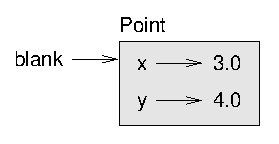
\includegraphics{figs/point.eps}}
\afterfig

The variable {\tt blank} refers to a Point object, which
contains two attributes.  Each attribute refers to a
floating-point number.

You can read the value of an attribute using the same syntax:

\beforeverb
\begin{verbatim}
>>> print blank.y
4.0
>>> x = blank.x
>>> print x
3.0
\end{verbatim}
\afterverb
%
The expression {\tt blank.x} means, ``Go to the object {\tt blank}
refers to and get the value of {\tt x}.'' In this case, we assign that
value to a variable named {\tt x}.  There is no conflict between
the variable {\tt x} and the attribute {\tt x}.

You can use dot notation as part of any expression.  For example:

\beforeverb
\begin{verbatim}
>>> print '(%g, %g)' % (blank.x, blank.y)
(3.0, 4.0)
>>> distance = math.sqrt(blank.x**2 + blank.y**2)
>>> print distance
5.0
\end{verbatim}
\afterverb
%
You can pass an instance as an argument in the usual way.
For example:

\index{instance!as argument}

\beforeverb
\begin{verbatim}
def print_point(p):
    print '(%g, %g)' % (p.x, p.y)
\end{verbatim}
\afterverb
%
\verb"print_point" takes a point as an argument and displays it in
mathematical notation.  To invoke it, you can pass {\tt blank} as
an argument:

\beforeverb
\begin{verbatim}
>>> print_point(blank)
(3.0, 4.0)
\end{verbatim}
\afterverb
%
Inside the function, {\tt p} is an alias for {\tt blank}, so if
the function modifies {\tt p}, {\tt blank} changes.

\index{aliasing}


\begin{ex}
Write a function called {\tt distance} that takes two Points
as arguments and returns the distance between them.
\end{ex}



\section{Rectangles}

Sometimes it is obvious what the attributes of an object should be,
but other times you have to make decisions.  For example, imagine you
are designing a class to represent rectangles.  What attributes would
you use to specify the location and size of a rectangle?  You can
ignore angle; to keep things simple, assume that the rectangle is
either vertical or horizontal.

\index{representation}

There are at least two possibilities: 

\begin{itemize}

\item You could specify one corner of the rectangle
(or the center), the width, and the height.

\item You could specify two opposing corners.

\end{itemize}

At this point it is hard to say whether either is better than
the other, so we'll implement the first one, just as an example.

\index{Rectangle class}
\index{class!Rectangle}

Here is the class definition:

\beforeverb
\begin{verbatim}
class Rectangle(object):
    """represent a rectangle. 
       attributes: width, height, corner.
    """
\end{verbatim}
\afterverb
%
The docstring lists the attributes:  {\tt width} and
{\tt height} are numbers; {\tt corner} is a Point object that
specifies the lower-left corner.

To represent a rectangle, you have to instantiate a Rectangle
object and assign values to the attributes:

\beforeverb
\begin{verbatim}
box = Rectangle()
box.width = 100.0
box.height = 200.0
box.corner = Point()
box.corner.x = 0.0
box.corner.y = 0.0
\end{verbatim}
\afterverb
%
The expression {\tt box.corner.x} means,
``Go to the object {\tt box} refers to and select the attribute named
{\tt corner}; then go to that object and select the attribute named
{\tt x}.''

The figure shows the state of this object:

\index{state diagram}
\index{diagram!state}
\index{object diagram}
\index{diagram!object}

\beforefig
\centerline{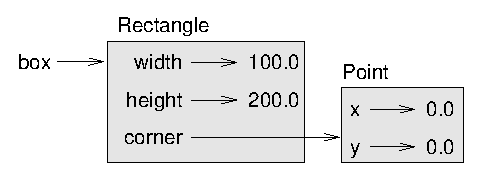
\includegraphics{figs/rectangle.eps}}
\afterfig

An object that is an attribute of another object is {\bf embedded}.

\index{embedded object}
\index{object!embedded}


\section{Instances as return values}

\index{instance!as return value}
\index{return value}

Functions can return instances.  For example, \verb"find_center"
takes a {\tt Rectangle} as an argument and returns a {\tt Point}
that contains the coordinates of the center of the {\tt Rectangle}:

\beforeverb
\begin{verbatim}
def find_center(box):
    p = Point()
    p.x = box.corner.x + box.width/2.0
    p.y = box.corner.y + box.height/2.0
    return p
\end{verbatim}
\afterverb
%
Here is an example that passes {\tt box} as an argument and assigns
the resulting Point to {\tt center}:

\beforeverb
\begin{verbatim}
>>> center = find_center(box)
>>> print_point(center)
(50.0, 100.0)
\end{verbatim}
\afterverb
%

\section{Objects are mutable}

\index{object!mutable}
\index{mutability}

You can change the state of an object by making an assignment to one of
its attributes.  For example, to change the size of a rectangle
without changing its position, you can modify the values of {\tt
width} and {\tt height}:

\beforeverb
\begin{verbatim}
box.width = box.width + 50
box.height = box.width + 100
\end{verbatim}
\afterverb
%
You can also write functions that modify objects.  For example,
\verb"grow_rectangle" takes a Rectangle object and two numbers,
{\tt dwidth} and {\tt dheight}, and adds the numbers to the
width and height of the rectangle:

\beforeverb
\begin{verbatim}
def grow_rectangle(rect, dwidth, dheight) :
    rect.width += dwidth
    rect.height += dheight
\end{verbatim}
\afterverb
%
Here is an example that demonstrates the effect:

\beforeverb
\begin{verbatim}
>>> print box.width
100.0
>>> print box.height
200.0
>>> grow_rectangle(box, 50, 100)
>>> print box.width
150.0
>>> print box.height
300.0
\end{verbatim}
\afterverb
%
Inside the function, {\tt rect} is an
alias for {\tt box}, so if the function modifies {\tt rect}, 
{\tt box} changes.

\begin{ex}
Write a function named \verb"move_rectangle" that takes
a Rectangle and two numbers named {\tt dx} and {\tt dy}.  It
should change the location of the rectangle by adding {\tt dx}
to the {\tt x} coordinate of {\tt corner} and adding {\tt dy}
to the {\tt y} coordinate of {\tt corner}.
\end{ex}


\section{Copying}

\index{aliasing}

Aliasing can make a program difficult to read because changes
in one place might have unexpected effects in another place.
It is hard to keep track of all the variables that might refer
to a given object.

\index{copying objects}
\index{object!copying}
\index{copy module}
\index{module!copy}

Copying an object is often an alternative to aliasing.
The {\tt copy} module contains a function called {\tt copy} that
can duplicate any object:

\beforeverb
\begin{verbatim}
>>> p1 = Point()
>>> p1.x = 3.0
>>> p1.y = 4.0

>>> import copy
>>> p2 = copy.copy(p1)
\end{verbatim}
\afterverb
%
{\tt p1} and {\tt p2} contain the same data, but they are
not the same Point.

\beforeverb
\begin{verbatim}
>>> print_point(p1)
(3.0, 4.0)
>>> print_point(p2)
(3.0, 4.0)
>>> p1 is p2
False
>>> p1 == p2
False
\end{verbatim}
\afterverb
%
The {\tt is} operator indicates that {\tt p1} and {\tt p2} are not the
same object, which is what we expected.  But you might have expected
{\tt ==} to yield {\tt True} because these points contain the same
data.  In that case, you will be disappointed to learn that for
instances, the default behavior of the {\tt ==} operator is the same
as the {\tt is} operator; it checks object identity, not object
equivalence.  This behavior can be changed---we'll see how later.

\index{is operator}
\index{operator!is}

If you use {\tt copy.copy} to duplicate a Rectangle, you will find
that it copies the Rectangle object but not the embedded Point.

\index{embedded object!copying}

\beforeverb
\begin{verbatim}
>>> box2 = copy.copy(box)
>>> box2 is box
False
>>> box2.corner is box.corner
True
\end{verbatim}
\afterverb
%
Here is what the object diagram looks like:

\index{state diagram}
\index{diagram!state}
\index{object diagram}
\index{diagram!object}

\vspace{0.1in}
\beforefig
\centerline{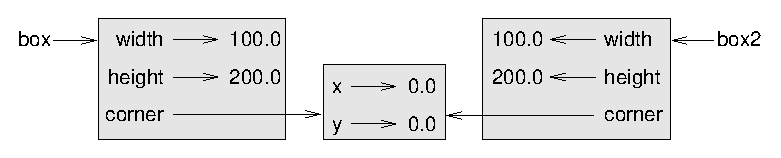
\includegraphics{figs/rectangle2.eps}}
\afterfig
\vspace{0.1in}

This operation is called a {\bf shallow copy} because it copies the
object and any references it contains, but not the embedded objects.

\index{shallow copy}
\index{copy!shallow}

For most applications, this is not what you want.  In this example,
invoking \verb"grow_rectangle" on one of the Rectangles would not
affect the other, but invoking \verb"move_rectangle" on either would
affect both!  This behavior is confusing and error-prone.

\index{deep copy}
\index{copy!deep}

Fortunately, the {\tt copy} module contains a method named {\tt
deepcopy} that copies not only the object but also 
the objects it refers to, and the objects {\em they} refer to,
and so on.
You will not be surprised to learn that this operation is
called a {\bf deep copy}.

\index{deepcopy function}
\index{function!deepcopy}

\beforeverb
\begin{verbatim}
>>> box3 = copy.deepcopy(box)
>>> box3 is box
False
>>> box3.corner is box.corner
False
\end{verbatim}
\afterverb
%
{\tt box3} and {\tt box} are completely separate objects.


\begin{ex}
Write a version of \verb"move_rectangle" that creates and
returns a new Rectangle instead of modifying the old one.
\end{ex}


\section{Debugging}
\label{hasattr}

\index{debugging}

When you start working with objects, you are likely to encounter
some new exceptions.  If you try to access an attribute
that doesn't exist, you get an {\tt AttributeError}:

\index{exception!AttributeError}
\index{AttributeError}

\beforeverb
\begin{verbatim}
>>> p = Point()
>>> print p.z
AttributeError: Point instance has no attribute 'z'
\end{verbatim}
\afterverb
%
If you are not sure what type an object is, you can ask:

\index{type function}
\index{function!type}

\beforeverb
\begin{verbatim}
>>> type(p)
<type '__main__.Point'>
\end{verbatim}
\afterverb
%
If you are not sure whether an object has a particular attribute,
you can use the built-in function {\tt hasattr}:

\index{hasattr function}
\index{function!hasattr}

\beforeverb
\begin{verbatim}
>>> hasattr(p, 'x')
True
>>> hasattr(p, 'z')
False
\end{verbatim}
\afterverb
%
The first argument can be any object; the second argument is a {\em
string} that contains the name of the attribute.


\section{Glossary}

\begin{description}

\item[class:] A user-defined type.  A class definition creates a new
class object.
\index{class}

\item[class object:] An object that contains information about a
user-defined type.  The class object can be used to create instances
of the type.
\index{class object}

\item[instance:] An object that belongs to a class.
\index{instance}

\item[attribute:] One of the named values associated with an object.
\index{attribute!instance}
\index{instance attribute}

\item[embedded (object):] An object that is stored as an attribute
of another object.
\index{embedded object}
\index{object!embedded}

\item[shallow copy:] To copy the contents of an object, including
any references to embedded objects;
implemented by the {\tt copy} function in the {\tt copy} module.
\index{shallow copy}

\item[deep copy:] To copy the contents of an object as well as any
embedded objects, and any objects embedded in them, and so on;
implemented by the {\tt deepcopy} function in the {\tt copy} module.
\index{deep copy}

\item[object diagram:] A diagram that shows objects, their
attributes, and the values of the attributes.
\index{object diagram}
\index{diagram!object}

\end{description}


\chapter{Classes and functions}
\label{time}


\section{Time}

As another example of a user-defined type, we'll define a class called
{\tt Time} that records the time of day.  The class definition looks
like this:

\index{user-defined type}
\index{type!user-defined}
\index{Time class}
\index{class!Time}

\beforeverb
\begin{verbatim}
class Time(object):
    """represents the time of day.
       attributes: hour, minute, second"""
\end{verbatim}
\afterverb
%
We can create a new {\tt Time} object and assign
attributes for hours, minutes, and seconds:

\beforeverb
\begin{verbatim}
time = Time()
time.hour = 11
time.minute = 59
time.second = 30
\end{verbatim}
\afterverb
%
The state diagram for the {\tt Time} object looks like this:

\index{state diagram}
\index{diagram!state}
\index{object diagram}
\index{diagram!object}

\beforefig
\centerline{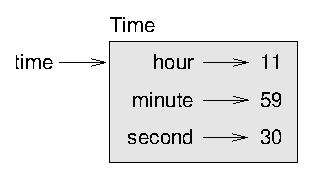
\includegraphics{figs/time.eps}}
\afterfig

\begin{ex}
\label{printtime}
Write a function called \verb"print_time" that takes a 
Time object and prints it in the form {\tt hour:minute:second}.
Hint: the format sequence \verb"'%.2d'" prints an integer using
at least two digits, including a leading zero if necessary.
\end{ex}

\begin{ex}
\label{is_after}

\index{boolean function}

Write a boolean function called \verb"is_after" that
takes two Time objects, {\tt t1} and {\tt t2}, and
returns {\tt True} if {\tt t1} follows {\tt t2} chronologically and
{\tt False} otherwise.  Challenge: don't use an {\tt if} statement.
\end{ex}


\section{Pure functions}

\index{prototype and patch}
\index{development plan!prototype and patch}

In the next few sections, we'll write two functions that add time
values.  They demonstrate two kinds of functions: pure functions and
modifiers.  They also demonstrate a development plan I'll call {\bf
  prototype and patch}, which is a way of tackling a complex problem
by starting with a simple prototype and incrementally dealing with the
complications.

Here is a simple prototype of \verb"add_time":

\beforeverb
\begin{verbatim}
def add_time(t1, t2):
    sum = Time()
    sum.hour = t1.hour + t2.hour
    sum.minute = t1.minute + t2.minute
    sum.second = t1.second + t2.second
    return sum
\end{verbatim}
\afterverb
%
The function creates a new {\tt Time} object, initializes its
attributes, and returns a reference to the new object.  This is called
a {\bf pure function} because it does not modify any of the objects
passed to it as arguments and it has no effect,
like displaying a value or getting user input, 
other than returning a value.

\index{pure function}
\index{function type!pure}

To test this function, I'll create two Time objects: {\tt start}
contains the start time of a movie, like {\em Monty Python and the
Holy Grail}, and {\tt duration} contains the run time of the movie,
which is one hour 35 minutes.

\index{Monty Python and the Holy Grail}

\verb"add_time" figures out when the movie will be done.

\beforeverb
\begin{verbatim}
>>> start = Time()
>>> start.hour = 9
>>> start.minute = 45
>>> start.second =  0

>>> duration = Time()
>>> duration.hour = 1
>>> duration.minute = 35
>>> duration.second = 0

>>> done = add_time(start, duration)
>>> print_time(done)
10:80:00
\end{verbatim}
\afterverb
%
The result, {\tt 10:80:00} might not be what you were hoping
for.  The problem is that this function does not deal with cases where the
number of seconds or minutes adds up to more than sixty.  When that
happens, we have to ``carry'' the extra seconds into the minute column
or the extra minutes into the hour column.

\index{carrying, addition with}

Here's an improved version:

\beforeverb
\begin{verbatim}
def add_time(t1, t2):
    sum = Time()
    sum.hour = t1.hour + t2.hour
    sum.minute = t1.minute + t2.minute
    sum.second = t1.second + t2.second

    if sum.second >= 60:
        sum.second -= 60
        sum.minute += 1

    if sum.minute >= 60:
        sum.minute -= 60
        sum.hour += 1

    return sum
\end{verbatim}
\afterverb
%
Although this function is correct, it is starting to get big.
We will see a shorter alternative later.


\section{Modifiers}
\label{increment}

\index{modifier}
\index{function type!modifier}

Sometimes it is useful for a function to modify the objects it gets as
parameters.  In that case, the changes are visible to the caller.
Functions that work this way are called {\bf modifiers}.

\index{increment}

{\tt increment}, which adds a given number of seconds to a {\tt Time}
object, can be written naturally as a
modifier.  Here is a rough draft:

\beforeverb
\begin{verbatim}
def increment(time, seconds):
    time.second += seconds

    if time.second >= 60:
        time.second -= 60
        time.minute += 1

    if time.minute >= 60:
        time.minute -= 60
        time.hour += 1
\end{verbatim}
\afterverb
%
The first line performs the basic operation; the remainder deals
with the special cases we saw before.

\index{special case}

Is this function correct?  What happens if the parameter {\tt seconds}
is much greater than sixty?  

In that case, it is not enough to carry
once; we have to keep doing it until {\tt time.second} is less than sixty.
One solution is to replace the {\tt if} statements with {\tt while}
statements.  That would make the function correct, but not
very efficient.

\begin{ex}
Write a correct version of {\tt increment} that
doesn't contain any loops.
\end{ex}

Anything that can be done with modifiers can also be done with pure
functions.  In fact, some programming languages only allow pure
functions.  There is some evidence that programs that use pure
functions are faster to develop and less error-prone than programs
that use modifiers.  But modifiers are convenient at times,
and functional programs tend to be less efficient.

In general, I recommend that you write pure functions whenever it is
reasonable and resort to modifiers only if there is a compelling
advantage.  This approach might be called a {\bf functional
programming style}.

\index{functional programming style}


\begin{ex}
Write a ``pure'' version of {\tt increment} that creates and returns
a new Time object rather than modifying the parameter.
\end{ex}


\section{Prototyping versus planning}
\label{prototype}

\index{prototype and patch}
\index{development plan!prototype and patch}
\index{planned development}
\index{development plan!planned}

The development plan I am demonstrating is called ``prototype and
patch.''  For each function, I wrote a prototype that performed the
basic calculation and then tested it, patching errors along the
way.

This approach can be effective, especially if you don't yet have a
deep understanding of the problem.  But incremental corrections can
generate code that is unnecessarily complicated---since it deals with
many special cases---and unreliable---since it is hard to know if you
have found all the errors.

An alternative is {\bf planned development}, in which high-level
insight into the problem can make the programming much easier.  In
this case, the insight is that a Time object is really a three-digit
number in base 60 (see \url{wikipedia.org/wiki/Sexagesimal})!  The
{\tt second} attribute is the ``ones column,'' the {\tt minute}
attribute is the ``sixties column,'' and the {\tt hour} attribute is
the ``thirty-six hundreds column.''

\index{sexagesimal}

When we wrote \verb"add_time" and {\tt increment}, we were effectively
doing addition in base 60, which is why we had to carry from one
column to the next.

\index{carrying, addition with}

This observation suggests another approach to the whole problem---we
can convert Time objects to integers and take advantage of the fact
that the computer knows how to do integer arithmetic.  

Here is a function that converts Times to integers:

\beforeverb
\begin{verbatim}
def time_to_int(time):
    minutes = time.hour * 60 + time.minute
    seconds = minutes * 60 + time.second
    return seconds
\end{verbatim}
\afterverb
%
And here is the function that converts integers to Times
(recall that {\tt divmod} divides the first argument by the second
and returns the quotient and remainder as a tuple).

\index{divmod}

\beforeverb
\begin{verbatim}
def int_to_time(seconds):
    time = Time()
    minutes, time.second = divmod(seconds, 60)
    time.hour, time.minute = divmod(minutes, 60)
    return time
\end{verbatim}
\afterverb
%
You might have to think a bit, and run some tests, to convince
yourself that these functions are correct.  One way to test them is to
check that \verb"time_to_int(int_to_time(x)) == x" for many values of
{\tt x}.  This is an example of a consistency check.

\index{consistency check}

Once you are convinced they are correct, you can use them to 
rewrite \verb"add_time":

\beforeverb
\begin{verbatim}
def add_time(t1, t2):
    seconds = time_to_int(t1) + time_to_int(t2)
    return int_to_time(seconds)
\end{verbatim}
\afterverb
%
This version is shorter than the original, and easier to verify.

\begin{ex}
Rewrite {\tt increment} using \verb"time_to_int" and \verb"int_to_time".
\end{ex}

In some ways, converting from base 60 to base 10 and back is harder
than just dealing with times.  Base conversion is more abstract; our
intuition for dealing with time values is better.

But if we have the insight to treat times as base 60 numbers and make
the investment of writing the conversion functions (\verb"time_to_int"
and \verb"int_to_time"), we get a program that is shorter, easier to
read and debug, and more reliable.

It is also easier to add features later.  For example, imagine
subtracting two Times to find the duration between them.  The
na\"{\i}ve approach would be to implement subtraction with borrowing.
Using the conversion functions would be easier and more likely to be
correct.

\index{subtraction with borrowing}
\index{borrowing, subtraction with}
\index{generalization}

Ironically, sometimes making a problem harder (or more general) makes it
easier (because there are fewer special cases and fewer opportunities
for error).


\section{Debugging}
\index{debugging}

A Time object is well-formed if the values of {\tt minutes} and {\tt
seconds} are between 0 and 60 (including 0 but not 60) and if 
{\tt hours} is positive.  {\tt hours} and {\tt minutes} should be
integral values, but we might allow {\tt seconds} to have a
fraction part.

\index{invariant}

These kind of requirements are called {\bf invariants} because
they should always be true.  To put it a different way, if they
are not true, then something has gone wrong.

Writing code to check your invariants can help you detect errors
and find their causes.  For example, you might have a function
like \verb"valid_time" that takes a Time object and returns
{\tt False} if it violates an invariant:

\beforeverb
\begin{verbatim}
def valid_time(time):
    if time.hours < 0 or time.minutes < 0 or time.seconds < 0:
        return False
    if time.minutes >= 60 or time.seconds >= 60:
        return False
    return True
\end{verbatim}
\afterverb
%
Then at the beginning of each function you could check the
arguments to make sure they are valid:

\index{raise statement}
\index{statement!raise}

\beforeverb
\begin{verbatim}
def add_time(t1, t2):
    if not valid_time(t1) or not valid_time(t2):
        raise ValueError, 'invalid Time object in add_time'
    seconds = time_to_int(t1) + time_to_int(t2)
    return int_to_time(seconds)
\end{verbatim}
\afterverb
%
Or you could use an {\tt assert} statement, which checks a given invariant
and raises an exception if it fails:

\index{assert statement}
\index{statement!assert}

\beforeverb
\begin{verbatim}
def add_time(t1, t2):
    assert valid_time(t1) and valid_time(t2)
    seconds = time_to_int(t1) + time_to_int(t2)
    return int_to_time(seconds)
\end{verbatim}
\afterverb
%
{\tt assert} statements are useful because they distinguish
code that deals with normal conditions from code
that checks for errors.


\section{Glossary}

\begin{description}

\item[prototype and patch:] A development plan that involves
writing a rough draft of a program, testing, and correcting errors as
they are found.
\index{prototype and patch}

\item[planned development:] A development plan that involves
high-level insight into the problem and more planning than incremental
development or prototype development.
\index{planned development}

\item[pure function:] A function that does not modify any of the objects it
receives as arguments.  Most pure functions are fruitful.
\index{pure function}

\item[modifier:] A function that changes one or more of the objects it
receives as arguments.  Most modifiers are fruitless.
\index{modifier}

\item[functional programming style:] A style of program design in which the
majority of functions are pure.
\index{functional programming style}

\item[invariant:] A condition that should always be true during the
execution of a program.
\index{invariant}

\end{description}


\section{Exercises}

\begin{ex}
Write a function called \verb"mul_time" that takes a Time object
and a number and returns a new Time object that contains
the product of the original Time and the number.

Then use \verb"mul_time" to write a function that takes a Time
object that represents the finishing time in a race, and a number
that represents the distance, and returns a Time object that represents
the average pace (time per mile).

\index{running pace}

\end{ex}

\begin{ex}

\index{Date class}
\index{class!Date}

Write a class definition for a Date object that has attributes {\tt
  day}, {\tt month} and {\tt year}.  Write a function called
\verb"increment_date" that takes a Date object, {\tt date} and an
integer, {\tt n}, and returns a new Date object that
represents the day {\tt n} days after {\tt date}.  Hint:
``Thirty days hath September...''  Challenge: does your function
deal with leap years correctly?  See \url{wikipedia.org/wiki/Leap_year}

\end{ex}


\begin{ex}

\index{datetime module}
\index{module!datetime}

The {\tt datetime} module provides {\tt date} and {\tt time} objects
that are similar to the Date and Time objects in this chapter, but
they provide a rich set of methods and operators.  Read the
documentation at \url{docs.python.org/lib/datetime-date.html}.

\begin{enumerate}

\item Use the {\tt datetime} module to write a program that
gets the current date and prints the day of the week.

\index{birthday}

\item Write a program that takes a birthday as input
and prints the user's age and the number of days, hours,
minutes and seconds until their next birthday.
\end{enumerate}

\end{ex}


\chapter{Classes and methods}


\section{Object-oriented features}

\index{object-oriented programming}

Python is an {\bf object-oriented programming language}, which means
that it provides features that support object-oriented
programming.

It is not easy to define object-oriented programming, but we have
already seen some of its characteristics:

\begin{itemize}

\item Programs are made up of object definitions and function
definitions, and most of the computation is expressed in terms
of operations on objects.

\item Each object definition corresponds to some object or concept
in the real world, and the functions that operate on that object
correspond to the ways real-world objects interact.

\end{itemize}

For example, the {\tt Time} class defined in Chapter~\ref{time}
corresponds to the way people record the time of day, and the
functions we defined correspond to the kinds of things people do with
times.  Similarly, the {\tt Point} and {\tt Rectangle} classes
correspond to the mathematical concepts of a point and a rectangle.

So far, we have not taken advantage of the features Python provides to
support object-oriented programming.  These
features are not strictly necessary; most of them provide
alternative syntax for things we have already done.  But in many cases,
the alternative is more concise and more accurately conveys the
structure of the program.

For example, in the {\tt Time} program, there is no obvious
connection between the class definition and the function definitions
that follow.  With some examination, it is apparent that every function
takes at least one {\tt Time} object as an argument.

\index{method}
\index{function}

This observation is the motivation for {\bf methods}; a method is
a function that is associated with a particular class.
We have seen methods for strings, lists, dictionaries and tuples.
In this chapter, we will define methods for user-defined types.

\index{syntax}
\index{semantics}

Methods are semantically the same as functions, but there are
two syntactic differences:

\begin{itemize}

\item Methods are defined inside a class definition in order
to make the relationship between the class and the method explicit.

\item The syntax for invoking a method is different from the
syntax for calling a function.

\end{itemize}

In the next few sections, we will take the functions from the previous
two chapters and transform them into methods.  This transformation is
purely mechanical; you can do it simply by following a sequence of
steps.  If you are comfortable converting from one form to another,
you will be able to choose the best form for whatever you are doing.


\section{Printing objects}
\label{print_time}

\index{object!printing}

In Chapter~\ref{time}, we defined a class named
{\tt Time} and in Exercise~\ref{printtime}, you 
wrote a function named \verb"print_time":

\beforeverb
\begin{verbatim}
class Time(object):
    """represents the time of day.
       attributes: hour, minute, second"""

def print_time(time):
    print '%.2d:%.2d:%.2d' % (time.hour, time.minute, time.second)
\end{verbatim}
\afterverb
%
To call this function, you have to pass a {\tt Time} object as an
argument:

\beforeverb
\begin{verbatim}
>>> start = Time()
>>> start.hour = 9
>>> start.minute = 45
>>> start.second = 00
>>> print_time(start)
09:45:00
\end{verbatim}
\afterverb
%
To make \verb"print_time" a method, all we have to do is
move the function definition inside the class definition.  Notice
the change in indentation.

\index{indentation}

\beforeverb
\begin{verbatim}
class Time(object):
    def print_time(time):
        print '%.2d:%.2d:%.2d' % (time.hour, time.minute, time.second)
\end{verbatim}
\afterverb
%
Now there are two ways to call \verb"print_time".  The first
(and less common) way is to use function syntax:

\index{function syntax}
\index{dot notation}


\beforeverb
\begin{verbatim}
>>> Time.print_time(start)
09:45:00
\end{verbatim}
\afterverb
%
In this use of dot notation, {\tt Time} is the name of the class,
and \verb"print_time" is the name of the method.  {\tt start} is
passed as a parameter.

The second (and more concise) way is to use method syntax:

\index{method syntax}

\beforeverb
\begin{verbatim}
>>> start.print_time()
09:45:00
\end{verbatim}
\afterverb
%
In this use of dot notation, \verb"print_time" is the name of the
method (again), and {\tt start} is the object the method is
invoked on, which is called the {\bf subject}.  Just as the
subject of a sentence is what the sentence is about, the subject
of a method invocation is what the method is about.

\index{subject}

Inside the method, the subject is assigned to the first
parameter, so in this case {\tt start} is assigned
to {\tt time}.

\index{self (parameter name)}
\index{parameter!self}

By convention, the first parameter of a method is
called {\tt self}, so it would be more common to write
\verb"print_time" like this:

\beforeverb
\begin{verbatim}
class Time(object):
    def print_time(self):
        print '%.2d:%.2d:%.2d' % (self.hour, self.minute, self.second)
\end{verbatim}
\afterverb
%
The reason for this convention is an implicit metaphor:

\index{metaphor, method invocation}

\begin{itemize}

\item The syntax for a function call, \verb"print_time(start)",
  suggests that the function is the active agent.  It says something
  like, ``Hey \verb"print_time"!  Here's an object for you to print.''

\item In object-oriented programming, the objects are the active
  agents.  A method invocation like \verb"start.print_time()" says
  ``Hey {\tt start}!  Please print yourself.''

\end{itemize}

This change in perspective might be more polite, but it is not obvious
that it is useful.  In the examples we have seen so far, it may not
be.  But sometimes shifting responsibility from the functions onto the
objects makes it possible to write more versatile functions, and makes
it easier to maintain and reuse code.

\begin{ex}
\label{convert}
Rewrite \verb"time_to_int"
(from Section~\ref{prototype}) as a method.  It is probably not
appropriate to rewrite \verb"int_to_time" as a method; it's not
clear what object you would invoke it on!
\end{ex}


\section{Another example}

\index{increment}

Here's a version of {\tt increment} (from Section~\ref{increment})
rewritten as a method:

\beforeverb
\begin{verbatim}
# inside class Time:

    def increment(self, seconds):
        seconds += self.time_to_int()
        return int_to_time(seconds)
\end{verbatim}
\afterverb
%
This version assumes that \verb"time_to_int" is written
as a method, as in Exercise~\ref{convert}.  Also, note that
it is a pure function, not a modifier.

Here's how you would invoke {\tt increment}:

\beforeverb
\begin{verbatim}
>>> start.print_time()
09:45:00
>>> end = start.increment(1337)
>>> end.print_time()
10:07:17
\end{verbatim}
\afterverb
%
The subject, {\tt start}, gets assigned to the first parameter,
{\tt self}.  The argument, {\tt 1337}, gets assigned to the
second parameter, {\tt seconds}.

This mechanism can be confusing, especially if you make an error.
For example, if you invoke {\tt increment} with two arguments, you
get:

\index{exception!TypeError}
\index{TypeError}

\beforeverb
\begin{verbatim}
>>> end = start.increment(1337, 460)
TypeError: increment() takes exactly 2 arguments (3 given)
\end{verbatim}
\afterverb
%
The error message is initially confusing, because there are
only two arguments in parentheses.  But the subject is also
considered an argument, so all together that's three.


\section{A more complicated example}

\verb"is_after" (from Exercise~\ref{is_after}) is slightly more complicated
because it takes two Time objects as parameters.  In this case it is
conventional to name the first parameter {\tt self} and the second
parameter {\tt other}:

\index{other (parameter name)}
\index{parameter!other}

\beforeverb
\begin{verbatim}
# inside class Time:

    def is_after(self, other):
        return self.time_to_int() > other.time_to_int()
\end{verbatim}
\afterverb
%
To use this method, you have to invoke it on one object and pass
the other as an argument:

\beforeverb
\begin{verbatim}
>>> end.is_after(start)
True
\end{verbatim}
\afterverb
%
One nice thing about this syntax is that it almost reads
like English: ``end is after start?''


\section{The init method}

\index{init method}
\index{method!init}

The init method (short for ``initialization'') is
a special method that gets invoked when an object is instantiated.  
Its full name is \verb"__init__" (two underscore characters,
followed by {\tt init}, and then two more underscores).  An
init method for the {\tt Time} class might look like this:

\beforeverb
\begin{verbatim}
# inside class Time:

    def __init__(self, hour=0, minute=0, second=0):
        self.hour = hour
        self.minute = minute
        self.second = second
\end{verbatim}
\afterverb
%
It is common for the parameters of \verb"__init__"
to have the same names as the attributes.  The statement

\beforeverb
\begin{verbatim}
        self.hour = hour
\end{verbatim}
\afterverb
%
stores the value of the parameter {\tt hour} as an attribute
of {\tt self}.

\index{optional parameter}
\index{parameter!optional}
\index{default value}
\index{override}

The parameters are optional, so if you call {\tt Time} with
no arguments, you get the default values.

\beforeverb
\begin{verbatim}
>>> time = Time()
>>> time.print_time()
00:00:00
\end{verbatim}
\afterverb
%
If you provide one argument, it overrides {\tt hour}:

\beforeverb
\begin{verbatim}
>>> time = Time (9)
>>> time.print_time()
09:00:00
\end{verbatim}
\afterverb
%
If you provide two arguments, they override {\tt hour} and
{\tt minute}.

\beforeverb
\begin{verbatim}
>>> time = Time(9, 45)
>>> time.print_time()
09:45:00
\end{verbatim}
\afterverb
%
And if you provide three arguments, they override all three
default values.


\begin{ex}
\index{Point class}
\index{class!Point}

Write an init method for the {\tt Point} class that takes
{\tt x} and {\tt y} as optional parameters and assigns
them to the corresponding attributes.
\end{ex}


\section{The {\tt \_\_str\_\_} method}

\index{str method@\_\_str\_\_ method}
\index{method!\_\_str\_\_}

\verb"__str__" is a special method, like \verb"__init__",
that is supposed to return a string representation of an object.

\index{string representation}

For example, here is a {\tt str} method for Time objects:

\beforeverb
\begin{verbatim}
# inside class Time:

    def __str__(self):
        return '%.2d:%.2d:%.2d' % (self.hour, self.minute, self.second)
\end{verbatim}
\afterverb
%
When you {\tt print} an object, Python invokes the {\tt str} method:

\index{print statement}
\index{statement!print}

\beforeverb
\begin{verbatim}
>>> time = Time(9, 45)
>>> print time
09:45:00
\end{verbatim}
\afterverb
%
When I write a new class, I almost always start by writing 
\verb"__init__", which makes it easier to instantiate objects, and 
\verb"__str__", which is useful for debugging.


\begin{ex}
Write a {\tt str} method for the {\tt Point} class.  Create
a Point object and print it.
\end{ex}


\section{Operator overloading}
\label{operator overloading}

By defining other special methods, you can specify the behavior
of operators on user-defined types.  For example, if you define
a method named \verb"__add__" for the {\tt Time} class, you can use the
{\tt +} operator on Time objects.

Here is what the definition might look like:

\index{add method}
\index{method!add}

\beforeverb
\begin{verbatim}
# inside class Time:

    def __add__(self, other):
        seconds = self.time_to_int() + other.time_to_int()
        return int_to_time(seconds)
\end{verbatim}
\afterverb
%
And here is how you could use it:

\beforeverb
\begin{verbatim}
>>> start = Time(9, 45)
>>> duration = Time(1, 35)
>>> print start + duration
11:20:00
\end{verbatim}
\afterverb
%
When you apply the {\tt +} operator to Time objects, Python invokes
\verb"__add__".  When you print the result, Python invokes 
\verb"__str__".  So there is quite a lot happening behind the scenes!

\index{operator overloading}

Changing the behavior of an operator so that it works with
user-defined types is called {\bf operator overloading}.  For every
operator in Python there is a corresponding special method, like 
\verb"__add__".  For more details, see
\url{docs.python.org/ref/specialnames.html}.

\begin{ex}
Write an {\tt add} method for the Point class.  
\end{ex}


\section{Type-based dispatch}

In the previous section we added two Time objects, but you
also might want to add an integer to a Time object.  The
following is a version of \verb"__add__"
that checks the type of {\tt other} and invokes either
\verb"add_time" or {\tt increment}:

\beforeverb
\begin{verbatim}
# inside class Time:

    def __add__(self, other):
        if isinstance(other, Time):
            return self.add_time(other)
        else:
            return self.increment(other)

    def add_time(self, other):
        seconds = self.time_to_int() + other.time_to_int()
        return int_to_time(seconds)

    def increment(self, seconds):
        seconds += self.time_to_int()
        return int_to_time(seconds)
\end{verbatim}
\afterverb
%
The built-in function {\tt isinstance} takes a value and a
class object, and returns {\tt True} if the value is an instance
of the class.

\index{isinstance function}
\index{function!isinstance}

If {\tt other} is a Time object, \verb"__add__" invokes
\verb"add_time".  Otherwise it assumes that the parameter
is a number and invokes {\tt increment}.  This operation is
called a {\bf type-based dispatch} because it dispatches the
computation to different methods based on the type of the
arguments.

\index{type-based dispatch}
\index{dispatch, type-based}

Here are examples that use the {\tt +} operator with different
types:

\beforeverb
\begin{verbatim}
>>> start = Time(9, 45)
>>> duration = Time(1, 35)
>>> print start + duration
11:20:00
>>> print start + 1337
10:07:17
\end{verbatim}
\afterverb
%
Unfortunately, this implementation of addition is not commutative.
If the integer is the first operand, you get

\index{commutativity}

\beforeverb
\begin{verbatim}
>>> print 1337 + start
TypeError: unsupported operand type(s) for +: 'int' and 'instance'
\end{verbatim}
\afterverb
%
The problem is, instead of asking the Time object to add an integer,
Python is asking an integer to add a Time object, and it doesn't know
how to do that.  But there is a clever solution for this problem: the
special method \verb"__radd__", which stands for ``right-side add.''
This method is invoked when a Time object appears on the right side of
the {\tt +} operator.  Here's the definition:

\index{radd method}
\index{method!radd}

\beforeverb
\begin{verbatim}
# inside class Time:

    def __radd__(self, other):
        return self.__add__(other)
\end{verbatim}
\afterverb
%
And here's how it's used:

\beforeverb
\begin{verbatim}
>>> print 1337 + start
10:07:17
\end{verbatim}
\afterverb
%

\begin{ex}
Write an {\tt add} method for Points that works with either a
Point object or a tuple:  

\begin{itemize}

\item If the second operand is a Point, the method should return a new
Point whose $x$ coordinate is the sum of the $x$ coordinates of the
operands, and likewise for the $y$ coordinates.

\item If the second operand is a tuple, the method should add the
first element of the tuple to the $x$ coordinate and the second
element to the $y$ coordinate, and return a new Point with the result. 

\end{itemize}

\end{ex}

\section{Polymorphism}

Type-based dispatch is useful when it is necessary, but (fortunately)
it is not always necessary.  Often you can avoid it by writing functions
that work correctly for arguments with different types.

\index{type-based dispatch}
\index{dispatch!type-based}

Many of the functions we wrote for strings will actually
work for any kind of sequence.
For example, in Section~\ref{histogram}
we used {\tt histogram} to count the number of times each letter
appears in a word.

\beforeverb
\begin{verbatim}
def histogram(s):
    d = dict()
    for c in s:
        if c not in d:
            d[c] = 1
        else:
            d[c] = d[c]+1
    return d
\end{verbatim}
\afterverb
%
This function also works for lists, tuples, and even dictionaries,
as long as the elements of {\tt s} are hashable, so they can be used
as keys in {\tt d}.

\beforeverb
\begin{verbatim}
>>> t = ['spam', 'egg', 'spam', 'spam', 'bacon', 'spam']
>>> histogram(t)
{'bacon': 1, 'egg': 1, 'spam': 4}
\end{verbatim}
\afterverb
%
Functions that can work with several types are called {\bf polymorphic}.
Polymorphism can facilitate code reuse.  For example, the built-in
function {\tt sum}, which adds the elements of a sequence, works
as long as the elements of the sequence support addition.

\index{polymorphism}

Since Time objects provide an {\tt add} method, they work
with {\tt sum}:

\beforeverb
\begin{verbatim}
>>> t1 = Time(7, 43)
>>> t2 = Time(7, 41)
>>> t3 = Time(7, 37)
>>> total = sum([t1, t2, t3])
>>> print total
23:01:00
\end{verbatim}
\afterverb
%
In general, if all of the operations inside a function 
work with a given type, then the function works with that type.

The best kind of polymorphism is the unintentional kind, where
you discover that a function you already wrote can be
applied to a type you never planned for.


\section{Debugging}
\index{debugging}

It is legal to add attributes to objects at any point in the execution
of a program, but if you are a stickler for type theory, it is a
dubious practice to have objects of the same type with different
attribute sets.  It is usually a good idea to
initialize all of an objects attributes in the init method.

\index{init method}
\index{attribute!initializing}

If you are not sure whether an object has a particular attribute, you
can use the built-in function {\tt hasattr} (see Section~\ref{hasattr}).

\index{hasattr function}
\index{function!hasattr}
\index{dict attribute@\_\_dict\_\_ attribute}
\index{attribute!\_\_dict\_\_}

Another way to access the attributes of an object is through the
special attribute \verb"__dict__", which is a dictionary that maps
attribute names (as strings) and values:

\beforeverb
\begin{verbatim}
>>> p = Point(3, 4)
>>> print p.__dict__
{'y': 4, 'x': 3}
\end{verbatim}
\afterverb
%
For purposes of debugging, you might find it useful to keep this
function handy:

\beforeverb
\begin{verbatim}
def print_attributes(obj):
    for attr in obj.__dict__:
        print attr, getattr(obj, attr)
\end{verbatim}
\afterverb
%
\verb"print_attributes" traverses the items in the object's dictionary
and prints each attribute name and its corresponding value.

\index{traversal!dictionary}
\index{dictionary!traversal}

The built-in function {\tt getattr} takes an object and an attribute
name (as a string) and returns the attribute's value.

\index{getattr function}
\index{function!getattr}


\section{Glossary}

\begin{description}

\item[object-oriented language:] A language that provides features,
  such as user-defined classes and method syntax, that facilitate
  object-oriented programming.
\index{object-oriented language}

\item[object-oriented programming:] A style of programming in which
data and the operations that manipulate it are organized into classes
and methods.
\index{object-oriented programming}

\item[method:] A function that is defined inside a class definition and
is invoked on instances of that class.
\index{method}

\item[subject:] The object a method is invoked on.
\index{subject}

\item[operator overloading:] Changing the behavior of an operator like
{\tt +} so it works with a user-defined type.
\index{overloading}
\index{operator!overloading}

\item[type-based dispatch:] A programming pattern that checks the type
of an operand and invokes different functions for different types.
\index{type-based dispatch}

\item[polymorphic:] Pertaining to a function that can work with more
  than one type.  

\index{polymorphism}

\end{description}

\section{Exercises}

\begin{ex}

\index{default value!avoiding mutable}
\index{mutable object, as default value}
\index{worst bug}
\index{bug!worst}

This exercise is a cautionary tale about one of the most
common, and difficult to find, errors in Python.

\begin{enumerate}

\index{Kangaroo class}
\index{class!Kangaroo}

\item Write a definition for a class named {\tt Kangaroo} with the following
methods:

\begin{enumerate}

\item An \verb"__init__" method that initializes an attribute named 
\verb"pouch_contents" to an empty list.

\item A method named \verb"put_in_pouch" that takes an object
of any type and adds it to \verb"pouch_contents".

\item A \verb"__str__" method that returns a string representation
of the Kangaroo object and the contents of the pouch.

\end{enumerate}
%
Test your code 
by creating two {\tt Kangaroo} objects, assigning them to variables
named {\tt kanga} and {\tt roo}, and then adding {\tt roo} to the
contents of {\tt kanga}'s pouch.

\item Download \url{thinkpython.com/code/BadKangaroo.py}.  It contains
a solution to the previous problem with one big, nasty bug.
Find and fix the bug.

If you get stuck, you can download
\url{thinkpython.com/code/GoodKangaroo.py}, which explains the
problem and demonstrates a solution.

\index{aliasing}
\index{embedded object}
\index{object!embedded}

\end{enumerate}


\end{ex}




\begin{ex}

\index{Visual module}
\index{module!Visual}
\index{vpython module}
\index{module!vpython}

Visual is a Python module that provides 3-D graphics.  It is
not always included in a Python installation, so you might have
to install it from your software repository or, if it's not there,
from \url{vpython.org}.

The following example creates a 3-D space that is 256 units
wide, long and high, and sets the ``center'' to be the
point $(128, 128, 128)$.  Then it draws a blue sphere.

\beforeverb
\begin{verbatim}
from visual import *

scene.range = (256, 256, 256)
scene.center = (128, 128, 128)

color = (0.1, 0.1, 0.9)          # mostly blue
sphere(pos=scene.center, radius=128, color=color)
\end{verbatim}
\afterverb

{\tt color} is an RGB tuple; that is, the elements are Red-Green-Blue
levels between 0.0 and 1.0 (see
\url{wikipedia.org/wiki/RGB_color_model}).

If you run this code, you should see a window with a black
background and a blue sphere.  If you drag the middle button
up and down, you can zoom in and out.  You can also rotate
the scene by dragging the right button, but with only one
sphere in the world, it is hard to tell the difference.

The following loop creates a cube of spheres:

\beforeverb
\begin{verbatim}
t = range(0, 256, 51)
for x in t:
    for y in t:
        for z in t:
            pos = x, y, z
            sphere(pos=pos, radius=10, color=color)
\end{verbatim}
\afterverb

\begin{enumerate}

\item Put this code in a script and make sure it works for
you.

\item Modify the program so that each sphere in the cube
has the color that corresponds to its position in RGB space.
Notice that the coordinates are in the range 0--255, but
the RGB tuples are in the range 0.0--1.0.

\index{color list}
\index{available colors}

\item Download \url{thinkpython.com/code/color_list.py}
and use the function \verb"read_colors" to generate a list
of the available colors on your system, their names and
RGB values.  For each named color draw a sphere in the
position that corresponds to its RGB values.



\end{enumerate}

You can see my solution at \url{thinkpython.com/code/color_space.py}.

\end{ex}


\chapter{Inheritance}

In this chapter we will develop classes to represent playing cards,
decks of cards, and poker hands.  If you don't play poker, you can
read about it at \url{wikipedia.org/wiki/Poker}, but you don't have
to; I'll tell you what you need to know for the exercises.

\index{playing card, Anglo-American}
\index{card, playing}
\index{poker}

If you are not familiar with Anglo-American playing cards,
you can read about them at \url{wikipedia.org/wiki/Playing_cards}.


\section{Card objects}

There are fifty-two cards in a deck, each of which belongs to one of
four suits and one of thirteen ranks.  The suits are Spades, Hearts,
Diamonds, and Clubs (in descending order in bridge).  The ranks are
Ace, 2, 3, 4, 5, 6, 7, 8, 9, 10, Jack, Queen, and King.  Depending on
the game that you are playing, an Ace may be higher than King
or lower than 2.

\index{rank}
\index{suit}

If we want to define a new object to represent a playing card, it is
obvious what the attributes should be: {\tt rank} and
{\tt suit}.  It is not as obvious what type the attributes
should be.  One possibility is to use strings containing words like
\verb"'Spade'" for suits and \verb"'Queen'" for ranks.  One problem with
this implementation is that it would not be easy to compare cards to
see which had a higher rank or suit.

\index{encode}
\index{encrypt}
\index{map to}
\index{representation}

An alternative is to use integers to {\bf encode} the ranks and suits.
In this context, ``encode'' means that we are going to define a mapping
between numbers and suits, or between numbers and ranks.  This
kind of encoding is not meant to be a secret (that
would be ``encryption'').

For example, this table shows the suits and the corresponding integer
codes:

\beforefig
\begin{tabular}{l c l}
Spades & $\mapsto$ & 3 \\
Hearts & $\mapsto$ & 2 \\
Diamonds & $\mapsto$ & 1 \\
Clubs & $\mapsto$ & 0
\end{tabular}
\afterfig

This code makes it easy to compare cards; because higher suits map to
higher numbers, we can compare suits by comparing their codes.

The mapping for ranks is fairly obvious; each of the numerical ranks
maps to the corresponding integer, and for face cards:

\beforefig
\begin{tabular}{l c l}
Jack & $\mapsto$ & 11 \\
Queen & $\mapsto$ & 12 \\
King & $\mapsto$ & 13 \\
\end{tabular}
\afterfig

I am using the $\mapsto$ symbol to make is clear that these mappings
are not part of the Python program.  They are part of the program
design, but they don't appear explicitly in the code.

\index{Card class}
\index{class!Card}

The class definition for {\tt Card} looks like this:

\beforeverb
\begin{verbatim}
class Card(object):
    """represents a standard playing card."""

    def __init__(self, suit=0, rank=2):
        self.suit = suit
        self.rank = rank
\end{verbatim}
\afterverb
%
As usual, the init method takes an optional
parameter for each attribute.  The default card is
the 2 of Clubs.

\index{init method}
\index{method!init}

To create a Card, you call {\tt Card} with the
suit and rank of the card you want.

\beforeverb
\begin{verbatim}
queen_of_diamonds = Card(1, 12)
\end{verbatim}
\afterverb
%


\section{Class attributes}

\index{class attribute}
\index{attribute!class}

In order to print Card objects in a way that people can easily
read, we need a mapping from the integer codes to the corresponding
ranks and suits.  A natural way to
do that is with lists of strings.  We assign these lists to {\bf class
attributes}:

\beforeverb
\begin{verbatim}
# inside class Card:

    suit_names = ['Clubs', 'Diamonds', 'Hearts', 'Spades']
    rank_names = [None, 'Ace', '2', '3', '4', '5', '6', '7', 
              '8', '9', '10', 'Jack', 'Queen', 'King']

    def __str__(self):
        return '%s of %s' % (Card.rank_names[self.rank],
                             Card.suit_names[self.suit])
\end{verbatim}
\afterverb
%
Variables like \verb"suit_names" and \verb"rank_names", which are
defined inside a class but outside of any method, are called
class attributes because they are associated with the class object 
{\tt Card}.

\index{instance attribute}
\index{attribute!instance}

This term distinguished them from variables like {\tt suit} and {\tt
  rank}, which are called {\bf instance attributes} because they are
associated with a particular instance.

\index{dot notation}

Both kinds of attribute are accessed using dot notation.  For
example, in \verb"__str__", {\tt self} is a Card object,
and {\tt self.rank} is its rank.  Similarly, {\tt Card}
is a class object, and \verb"Card.rank_names" is a
list of strings associated with the class.

Every card has its own {\tt suit} and {\tt rank}, but there
is only one copy of \verb"suit_names" and \verb"rank_names".

Putting it all together, the expression
\verb"Card.rank_names[self.rank]" means ``use the attribute {\tt rank}
from the object {\tt self} as an index into the list \verb"rank_names"
from the class {\tt Card}, and select the appropriate string.''

The first element of \verb"rank_names" is {\tt None} because there
is no card with rank zero.  By including {\tt None} as a place-keeper,
we get a mapping with the nice property that the index 2 maps to the
string \verb"'2'", and so on.  To avoid this tweak, we could have
used a dictionary instead of a list.

With the methods we have so far, we can create and print cards:

\beforeverb
\begin{verbatim}
>>> card1 = Card(2, 11)
>>> print card1
Jack of Hearts
\end{verbatim}
\afterverb
%
Here is a diagram that shows the {\tt Card} class object
and one Card instance:

\index{state diagram}
\index{diagram!state}
\index{object diagram}
\index{diagram!object}

\beforefig
\centerline{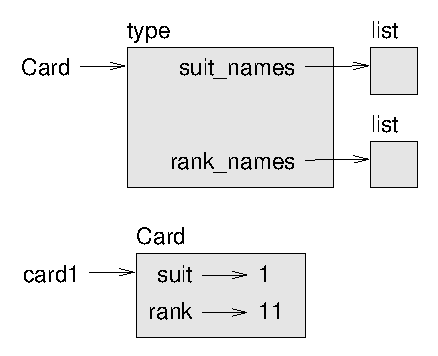
\includegraphics{figs/card1.eps}}
\afterfig

{\tt Card} is a class object, so it has type {\tt type}.  {\tt
card1} has type {\tt Card}.  (To save space, I didn't draw the
contents of \verb"suit_names" and \verb"rank_names").


\section{Comparing cards}
\label{comparecard}

\index{operator!conditional}
\index{conditional operator}

For built-in types, there are conditional operators
({\tt <}, {\tt >}, {\tt ==}, etc.)
that compare
values and determine when one is greater than, less than, or equal to
another.  For user-defined types, we can override the behavior of
the built-in operators by providing a method named
\verb"__cmp__".  

\verb"__cmp__" takes two parameters, {\tt self} and {\tt other},
and returns a positive number if the first object is greater, a
negative number if the second object is greater, and 0 if they are
equal to each other.

\index{override}
\index{operator overloading}

The correct ordering for cards is not obvious.
For example, which
is better, the 3 of Clubs or the 2 of Diamonds?  One has a higher
rank, but the other has a higher suit.  In order to compare
cards, you have to decide whether rank or suit is more important.

The answer might depend on what game you are playing, but to keep
things simple, we'll make the arbitrary choice that suit is more
important, so all of the Spades outrank all of the Diamonds,
and so on.

\index{cmp method@\_\_cmp\_\_ method}
\index{method!\_\_cmp\_\_}

With that decided, we can write \verb"__cmp__":

\beforeverb
\begin{verbatim}
# inside class Card:

    def __cmp__(self, other):
        # check the suits
        if self.suit > other.suit: return 1
        if self.suit < other.suit: return -1

        # suits are the same... check ranks
        if self.rank > other.rank: return 1
        if self.rank < other.rank: return -1

        # ranks are the same... it's a tie
        return 0    
\end{verbatim}
\afterverb
%
You can write this more concisely using tuple comparison:

\index{tuple!comparison}
\index{comparison!tuple}

\beforeverb
\begin{verbatim}
# inside class Card:

    def __cmp__(self, other):
        t1 = self.suit, self.rank
        t2 = other.suit, other.rank
        return cmp(t1, t2)
\end{verbatim}
\afterverb
%
The built-in function {\tt cmp} has the same interface as
the method \verb"__cmp__": it takes two values and returns
a positive number if the first is larger, a negative number
if the second is larger, and 0 if they are equal.

\index{cmp function}
\index{function!cmp}


\begin{ex}
Write a \verb"__cmp__" method for Time objects.  Hint: you
can use tuple comparison, but you also might consider using
integer subtraction.

%    def __cmp__(self, other):
%        return time_to_int(self) - time_to_int(other)

%If {\tt self} is later than {\tt other}, the result is
%a positive number.  If {\tt other} is later, the result
%is negative.  And if {\tt self} and {\tt other} are equal
%(but not necessarily identical)
%the result is zero.

\end{ex}


\section{Decks}
\index{list!of objects}
\index{deck, playing cards}

Now that we have Cards, the next step is to define Decks.  Since a
deck is made up of cards, it is natural for each Deck to contain a
list of cards as an attribute.

\index{init method}
\index{method!init}

The following is a class definition for {\tt Deck}.  The
init method creates the attribute {\tt cards} and generates
the standard set of fifty-two cards:

\index{composition}
\index{loop!nested}

\index{Deck class}
\index{class!Deck}

\beforeverb
\begin{verbatim}
class Deck(object):

    def __init__(self):
        self.cards = []
        for suit in range(4):
            for rank in range(1, 14):
                card = Card(suit, rank)
                self.cards.append(card)
\end{verbatim}
\afterverb
%
The easiest way to populate the deck is with a nested loop.  The outer
loop enumerates the suits from 0 to 3.  The inner loop enumerates the
ranks from 1 to 13.  Each iteration
creates a new Card with the current suit and rank,
and appends it to {\tt self.cards}.

\index{append method}
\index{method!append}


\section{Printing the deck}
\label{printdeck}

\index{str method@\_\_str\_\_ method}
\index{method!\_\_str\_\_}

Here is a \verb"__str__" method for {\tt Deck}:

\beforeverb
\begin{verbatim}
#inside class Deck:

    def __str__(self):
        res = []
        for card in self.cards:
            res.append(str(card))
        return '\n'.join(res)
\end{verbatim}
\afterverb
%
This method demonstrates an efficient way to accumulate a large
string: building a list of strings and then using {\tt join}.
The built-in function {\tt str} invokes the \verb"__str__"
method on each card and returns the string representation.

\index{accumulator!string}
\index{string!accumulator}
\index{join method}
\index{method!join}
\index{newline}

Since we invoke {\tt join} on a newline character, the cards
are separated by newlines.  Here's what the result looks like:

\beforeverb
\begin{verbatim}
>>> deck = Deck()
>>> print deck
Ace of Clubs
2 of Clubs
3 of Clubs
...
10 of Spades
Jack of Spades
Queen of Spades
King of Spades
\end{verbatim}
\afterverb
%
Even though the result appears on 52 lines, it is
one long string that contains newlines.


\section{Add, remove, shuffle and sort}

To deal cards, we would like a method that
removes a card from the deck and returns it.
The list method {\tt pop} provides a convenient way to do that:

\index{pop method}
\index{method!pop}

\beforeverb
\begin{verbatim}
#inside class Deck:

    def pop_card(self):
        return self.cards.pop()
\end{verbatim}
\afterverb
%
Since {\tt pop} removes the {\em last} card in the list, we are
dealing from the bottom of the deck.  In real life bottom dealing is
frowned upon\footnote{See \url{wikipedia.org/wiki/Bottom_dealing}.},
but in this context it's ok.

\index{append method}
\index{method!append}

To add a card, we can use the list method {\tt append}:

\beforeverb
\begin{verbatim}
#inside class Deck:

    def add_card(self, card):
        self.cards.append(card)
\end{verbatim}
\afterverb
%
A method like this that uses another function without doing
much real work is sometimes called a {\bf veneer}.  The metaphor
comes from woodworking, where it is common to glue a thin
layer of good quality wood to the surface of a cheaper piece of
wood.

\index{veneer}

In this case we are defining a ``thin'' method that expresses
a list operation in terms that are appropriate for decks.

As another example, we can write a Deck method named {\tt shuffle}
using the function {\tt shuffle} from the {\tt random} module:

\index{random module}
\index{module!random}
\index{shuffle function}
\index{function!shuffle}

\beforeverb
\begin{verbatim}
# inside class Deck:
            
    def shuffle(self):
        random.shuffle(self.cards)
\end{verbatim}
\afterverb
%
Don't forget to import {\tt random}.

\begin{ex}
\index{sort method}
\index{method!sort}

Write a Deck method named {\tt sort} that uses the list method
{\tt sort} to sort the cards in a {\tt Deck}.  {\tt sort} uses
the \verb"__cmp__" method we defined to determine sort order.
\end{ex}



\section{Inheritance}

\index{inheritance}
\index{object-oriented programming}

The language feature most often associated with object-oriented
programming is {\bf inheritance}.  Inheritance is the ability to
define a new class that is a modified version of an existing
class.

\index{parent class}
\index{child class}
\index{class!child}
\index{subclass}
\index{superclass}

It is called ``inheritance'' because the new class inherits the
methods of the existing class.  Extending this metaphor, the existing
class is called the {\bf parent} and the new class is
called the {\bf child}.

As an example, let's say we want a class to represent a ``hand,''
that is, the set of cards held by one player.  A hand is similar to a
deck: both are made up of a set of cards, and both require operations
like adding and removing cards.

A hand is also different from a deck; there are operations we want for
hands that don't make sense for a deck.  For example, in poker we
might compare two hands to see which one wins.  In bridge, we might
compute a score for a hand in order to make a bid.

This relationship between classes---similar, but different---lends
itself to inheritance.  

The definition of a child class is like other class definitions,
but the name of the parent class appears in parentheses:

\index{parentheses!parent class in}
\index{parent class}
\index{class!parent}
\index{Hand class}
\index{class!Hand}

\beforeverb
\begin{verbatim}
class Hand(Deck):
    """represents a hand of playing cards"""
\end{verbatim}
\afterverb
%
This definition indicates that {\tt Hand} inherits from {\tt Deck};
that means we can use methods like \verb"pop_card" and \verb"add_card"
for Hands as well as Decks.

{\tt Hand} also inherits \verb"__init__" from {\tt Deck}, but
it doesn't really do what we want: instead of populating the hand
with 52 new cards, the init method for Hands should initialize
{\tt cards} with an empty list.

\index{override}
\index{init method}
\index{method!init}

If we provide an init method in the {\tt Hand} class, it overrides the
one in the {\tt Deck} class:

\beforeverb
\begin{verbatim}
# inside class Hand:

    def __init__(self, label=''):
        self.cards = []
        self.label = label
\end{verbatim}
\afterverb
%
So when you create a Hand, Python invokes this init method:

\beforeverb
\begin{verbatim}
>>> hand = Hand('new hand')
>>> print hand.cards
[]
>>> print hand.label
new hand
\end{verbatim}
\afterverb
%
But the other methods are inherited from {\tt Deck}, so we can use
\verb"pop_card" and \verb"add_card" to deal a card:

\beforeverb
\begin{verbatim}
>>> deck = Deck()
>>> card = deck.pop_card()
>>> hand.add_card(card)
>>> print hand
King of Spades
\end{verbatim}
\afterverb
%
A natural next step is to encapsulate this code in a method
called \verb"move_cards":

\index{encapsulation}

\beforeverb
\begin{verbatim}
#inside class Deck:

    def move_cards(self, hand, num):
        for i in range(num):
            hand.add_card(self.pop_card())
\end{verbatim}
\afterverb
%
\verb"move_cards" takes two arguments, a Hand object and the number of
cards to deal.  It modifies both {\tt self} and {\tt hand}, and
returns {\tt None}.

In some games, cards are moved from one hand to another,
or from a hand back to the deck.  You can use \verb"move_cards"
for any of these operations: {\tt self} can be either a Deck
or a Hand, and {\tt hand}, despite the name, can also be a {\tt Deck}.

\begin{ex}
Write a Deck method called \verb"deal_hands" that takes two
parameters, the number of hands and the number of cards per
hand, and that creates new Hand objects, deals the appropriate
number of cards per hand, and returns a list of Hand objects.
\end{ex}

Inheritance is a useful feature.  Some programs that would be
repetitive without inheritance can be written more elegantly
with it.  Inheritance can facilitate code reuse, since you can
customize the behavior of parent classes without having to modify
them.  In some cases, the inheritance structure reflects the natural
structure of the problem, which makes the program easier to
understand.

On the other hand, inheritance can make programs difficult to read.
When a method is invoked, it is sometimes not clear where to find its
definition.  The relevant code may be scattered among several modules.
Also, many of the things that can be done using inheritance can be
done as well or better without it.  


\section{Class diagrams}

So far we have seen stack diagrams, which show the state of
a program, and object diagrams, which show the attributes
of an object and their values.  These diagrams represent a snapshot
in the execution of a program, so they change as the program
runs.

They are also highly detailed; for some purposes, too
detailed.  A class diagrams is a more abstract representation
of the structure of a program.  Instead of showing individual
objects, it shows classes and the relationships between them.

There are several kinds of relationship between classes:

\begin{itemize}

\item Objects in one class might contain references to objects
in another class.  For example, each Rectangle contains a reference
to a Point, and each Deck contains references to many Cards.
This kind of relationship is called {\bf HAS-A}, as in, ``a Rectangle
has a Point.''

\item One class might inherit from another.  This relationship
is called {\bf IS-A}, as in, ``a Hand is a kind of a Deck.''

\item One class might depend on another in the sense that changes
in one class would require changes in the other.

\end{itemize}

\index{IS-A relationship}
\index{HAS-A relationship}
\index{class diagram}
\index{diagram!class}
\index{UML}

A {\bf class diagram} is a graphical representation of these
relationships\footnote{The diagrams I am using here are similar to UML
  (see \url{wikipedia.org/wiki/Unified_Modeling_Language}), with a few
  simplifications.}.  For example, this diagram shows the
relationships between {\tt Card}, {\tt Deck} and {\tt Hand}.

\beforefig
\centerline{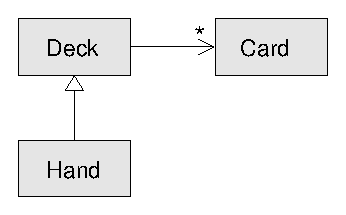
\includegraphics{figs/class1.eps}}
\afterfig

The arrow with a hollow triangle head represents an IS-A
relationship; in this case it indicates that Hand inherits
from Deck.

The standard arrow head represents a HAS-A
relationship; in this case a Deck has references to Card
objects.

\index{multiplicity (in class diagram)}

The star ({\tt *}) near the arrow head is a 
{\bf multiplicity}; it indicates how many Cards a Deck has.
A multiplicity can be a simple number, like {\tt 52}, a range,
like {\tt 5..7} or a star, which indicates that a Deck can
have any number of Cards.

A more detailed diagram might show that a Deck actually
contains a {\em list} of Cards, but built-in types
like list and dict are usually not included in class diagrams.


\section{Debugging}
\index{debugging}

Inheritance can make debugging a challenge because when you
invoke a method on an object, you might not know which method
will be invoked.

\index{polymorphism}

Suppose you are writing a function that works with Hand objects.
You would like it to work with all kinds of Hands, like
PokerHands, BridgeHands, etc.  If you invoke a method like
{\tt shuffle}, you might get the one defined in {\tt Deck},
but if any of the subclasses override this method, you'll
get that version instead.  

\index{flow of execution}

Any time you are unsure about the flow of execution through your
program, the simplest solution is to add print statements at the
beginning of the relevant methods.  If {\tt Deck.shuffle} prints a
message that says something like {\tt Running Deck.shuffle}, then as
the program runs it traces the flow of execution.

As an alternative, you could use this function, which takes an
object and a method name (as a string) and returns the class that
provides the definition of the method:

\beforeverb
\begin{verbatim}
def find_defining_class(obj, meth_name):
    for ty in type(obj).mro():
        if meth_name in ty.__dict__:
            return ty
\end{verbatim}
\afterverb
%
Here's an example:

\beforeverb
\begin{verbatim}
>>> hand = Hand()
>>> print find_defining_class(hand, 'shuffle')
<class 'Card.Deck'>
\end{verbatim}
\afterverb
%
So the {\tt shuffle} method for this Hand is the one in {\tt Deck}.

\index{mro method}
\index{method!mro}
\index{method resolution order}

\verb"find_defining_class" uses the {\tt mro} method to get the list
of class objects (types) that will be searched for methods.  ``MRO''
stands for ``method resolution order.''

\index{override}
\index{interface}
\index{precondition}
\index{postcondition}

Here's a program design suggestion: whenever you override a method,
the interface of the new method should be the same as the old.  It
should take the same parameters, return the same type, and obey the
same preconditions and postconditions.  If you obey this rule, you
will find that any function designed to work with an instance of a
superclass, like a Deck, will also work with instances of subclasses
like a Hand or PokerHand.

If you violate this rule, your code will collapse like (sorry)
a house of cards.


\section{Glossary}

\begin{description}

\item[encode:]  To represent one set of values using another
set of values by constructing a mapping between them.
\index{encode}

\item[class attribute:] An attribute associated with a class
object.  Class attributes are defined inside
a class definition but outside any method.
\index{class attribute}
\index{attribute!class}

\item[instance attribute:] An attribute associated with an
instance of a class.
\index{instance attribute}
\index{attribute!instance}

\item[veneer:] A method or function that provides a different
interface to another function without doing much computation.
\index{veneer}

\item[inheritance:] The ability to define a new class that is a
modified version of a previously defined class.
\index{inheritance}

\item[parent class:] The class from which a child class inherits.
\index{parent class}

\item[child class:] A new class created by inheriting from an
existing class; also called a ``subclass.''
\index{child class}
\index{class!child}

\item[IS-A relationship:] The relationship between a child class
and its parent class.
\index{IS-A relationship}

\item[HAS-A relationship:] The relationship between two classes
where instances of one class contain references to instances of
the other.
\index{HAS-A relationship}

\item[class diagram:] A diagram that shows the classes in a program
and the relationships between them.
\index{class diagram}
\index{diagram!class}

\item[multiplicity:] A notation in a class diagram that shows, for
a HAS-A relationship, how many references there are to instances
of another class.
\index{multiplicity (in class diagram)}

\end{description}


\section{Exercises}

\begin{ex}
\index{poker}


The following are the possible hands in poker, in increasing order
of value (and decreasing order of probability):

\begin{description}

\item[pair:] two cards with the same rank
\vspace{-0.05in}

\item[two pair:] two pairs of cards with the same rank
\vspace{-0.05in}

\item[three of a kind:] three cards with the same rank
\vspace{-0.05in}

\item[straight:] five cards with ranks in sequence (aces can
be high or low, so {\tt Ace-2-3-4-5} is a straight and so is {\tt
10-Jack-Queen-King-Ace}, but {\tt Queen-King-Ace-2-3} is not.)
\vspace{-0.05in}

\item[flush:] five cards with the same suit
\vspace{-0.05in}

\item[full house:] three cards with one rank, two cards with another
\vspace{-0.05in}

\item[four of a kind:] four cards with the same rank
\vspace{-0.05in}

\item[straight flush:] five cards in sequence (as defined above) and
with the same suit
\vspace{-0.05in}

\end{description}
%
The goal of these exercises is to estimate
the probability of drawing these various hands.

\begin{enumerate}

\item Download the following files from \url{thinkpython.com/code}:

\begin{description}

\item[{\tt Card.py}]: A complete version of the {\tt Card},
{\tt Deck} and {\tt Hand} classes in this chapter.

\item[{\tt PokerHand.py}]: An incomplete implementation of a class
that represents a poker hand, and some code that tests it.

\end{description}
%
\item If you run {\tt PokerHand.py}, it deals seven 7-card poker hands
and checks to see if any of them contains a flush.  Read this
code carefully before you go on.

\item Add methods to {\tt PokerHand.py} named \verb"has_pair",
\verb"has_twopair", etc. that return True or False according to
whether or not the hand meets the relevant criteria.  Your code should
work correctly for ``hands'' that contain any number of cards
(although 5 and 7 are the most common sizes).

\item Write a method named {\tt classify} that figures out
the highest-value classification for a hand and sets the
{\tt label} attribute accordingly.  For example, a 7-card hand
might contain a flush and a pair; it should be labeled ``flush''.

\item When you are convinced that your classification methods are
working, the next step is to estimate the probabilities of the various
hands.  Write a function in {\tt PokerHand.py} that shuffles a deck of
cards, divides it into hands, classifies the hands, and counts the
number of times various classifications appear.

\item Print a table of the classifications and their probabilities.
Run your program with larger and larger numbers of hands until the
output values converge to a reasonable degree of accuracy.  Compare
your results to the values at \url{wikipedia.org/wiki/Hand_rankings}.

\end{enumerate}
\end{ex}
